\section{Casimir forces between a conducting plate and a dielectric sphere}
\label{sec:3:casimir-plate-sphere}

An empirical derivation for power law of the casimir energy between a sphere and a conducting plate can be made directly from the energy between two atoms with static polarizability $\alpha_i$ given by Casimir and Polder \cite{Casimir_1948a}. They derived an expression for the Casimir-Polder potential of \footnote{For two macroscopic spheres, the casimir potential looks very similar to eq. \eqref{eq:3:casimir-polder-atom-atom}. The polarizability of a sphere is given by eq. \eqref{eq:3:polarizability-sphere}. Using this result, the Casimir energy between two identical dielectric spheres in the large separation limit is given as $-\frac{23\hbar c}{4\pi L^7}\left(\frac{\varepsilon_r-1}{\varepsilon_r+2}\right)^2R^6$ \cite{Emig_2007}.}
\begin{equation}\label{eq:3:casimir-polder-atom-atom}
  E = -\frac{23\hbar c \alpha_1 \alpha_2}{4 \pi L^7} .
\end{equation}
The polarizability of a sphere with radius $R$ is derived in appendix \ref{apx:polarizability-sphere} and is given for an dielectric with $\varepsilon_r$ as 
\begin{equation} \label{eq:3:polarizability-sphere}
  \alpha_\mathrm{sphere} \propto \left(\frac{\varepsilon_r-1}{\varepsilon_r+2}\right)R^3 .
\end{equation}
If one atom is now replaced by a conducting sphere ($\varepsilon_r \rightarrow \infty$) of radius $\sim L$ (much larger than the atom) with a polarizability of $L^3$, it get obvious that between this big sphere and the atom, the energy is given by a power law of $1/L^4$.
It is therefore natural to assume, that for a macroscopic sphere and a macroscopic plate, the Casimir energy behaves similar to a $1/L^4$ law - at least for the \emph{large separation limit (LSL)}.
The exact calculation for this problem is very hard. In fact, no analytic solution is known.

Ford was able to determine an integral expression using a macroscopic approach in 1998 \cite{Ford_1998}:
\begin{multline}
  F = - \frac{\hbar c}{4 \pi L^4} \int_{0}^{\infty} \dd \omega \, \alpha(\omega) \left[3\sin 2 \omega L - 6L\omega \cos 2 \omega L \right. \\ 
  \left. - 6L^2\omega^2 \sin 2 \omega L + 4L^3\omega^3 \cos 2 \omega L\right].
\end{multline}
The expression depends on the polarizability, which is generally not constant for a dielectric. Especially for small separations between the sphere and the plate, this dependence and the non-constant polarizability make this integral nearly unsolvable.
For large separations, much larger than the absorption wavelength of the dielectric or much larger than the wavelength corresponding to the plasma frequency in the Drude-Model, the polarizability can be assumed to be static $\alpha=\mathrm{const}$ \cite{Ford_1998,Kamp_2020}. In this simplifying case, the integral can be solved using an exponential convergence factor and results in
\begin{equation}
  F = -\frac{6 \hbar c}{4 \pi L^5} \alpha
\end{equation}
and thus 
\begin{equation}\label{eq:3:casimir-sphere-plate}
  E = -\frac{3}{8}\frac{\hbar c}{\pi L^4} \left(\frac{\varepsilon_r - 1}{\varepsilon_r + 2}\right)R^3 .
\end{equation}
For the large separations, the Casimir interaction between a sphere and a plate indeed behaves like expected compared with the motivation of the $1/L^4$-law above in this section.

A second method to calculate the Casimir energy for arbitrary compact objects and a conducting wall was developed in Ref. \cite{Emig_2007}. For the sphere-plate geometry, this results in the large separation limit (LSL) in a infinite series, where the first-order term ($\propto 1/L^4$) is precisely given by eq. \eqref{eq:3:casimir-sphere-plate} \cite{Emig_2007a,Pirozhenko_2013}. The first 8 terms of this series are shown in \cref{fig:3:casimir-behavior} as well as a few specific numerical points for higher terms.
\begin{figure}[!ht]
  \centering
  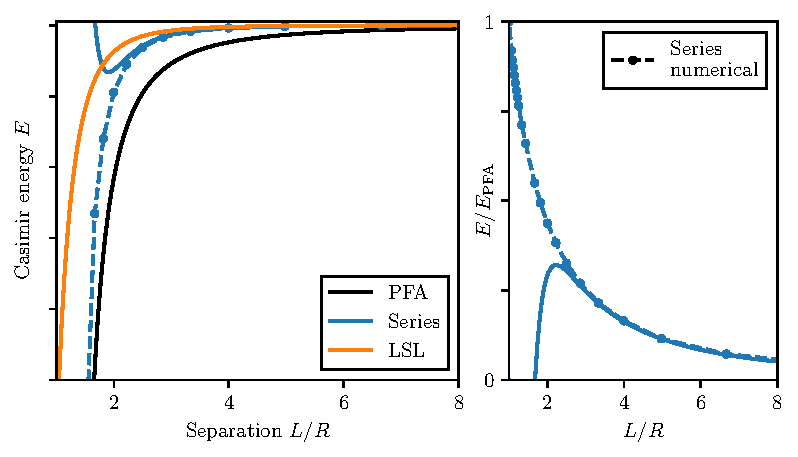
\includegraphics[width=\textwidth]{./../figures/casimir/casimir-behavior.pdf}
  \caption{Behavior of different approximations of the casimir interaction between a conducting sphere and a perfectly conducting plate. Additionally, a comparison between the PFA and an exact numerical series expansion from Ref. \cite{Emig_2007a} is shown.}
  \label{fig:3:casimir-behavior}
\end{figure}
It becomes evident, that the series expansion converges to the LSL eq. \eqref{eq:3:casimir-sphere-plate} for large separations and to the PFA eq. \eqref{eq:3:PFA-sphere-plate} for small separations.
However, quantitatively the numerics show, that $E/E_\mathrm{PFA} \leq 1$ and thus the PFA predicts a stronger Casimir energy for all separations.

\begin{theorem}
  The PFA model for the Casimir energy between a conducting sphere and a conducting plate is an upper bound for the actual Casimir potential for any separation $L/R$.
\end{theorem}
\begin{proof}
  The proof is given in the following two steps: First it is shown that \textbf{(a)} $\abs{E_\mathrm{PFA}} > \abs{E_\mathrm{LSL}}$ for arbitrary dielectric spheres, then it is shown that \textbf{(b)} $\abs{E_\mathrm{PFA,\,cond.}} \geq \abs{E_\mathrm{PFA\,diel.}}$. Using the numerical series expansion in \cref{fig:3:casimir-behavior} it is clear that this argumentation holds for all separations $L/R$.
  
  \textbf{(a)} Directly comparing the PFA eq. \eqref{eq:3:PFA-sphere-plate} and the LSL eq. \eqref{eq:3:casimir-sphere-plate} shows
  \begin{align}
    \abs{E_\mathrm{PFA}} &> \abs{E_\mathrm{LSL}}\\
    \frac{\hbar c \pi^3}{720} \left(\frac{\varepsilon_r - 1}{\varepsilon_r + 1}\right)\varphi(\varepsilon_r) \frac{R}{\mathscr{L}^2} &> \frac{3\hbar c}{8 \pi L^4}\left(\frac{\varepsilon_r - 1}{\varepsilon_r + 2}\right) R^3 \\
    \frac{8 \pi^4}{3 \cdot 720} \frac{\varepsilon_r + 2}{\varepsilon_r + 1} \varphi(\varepsilon_r) &> \frac{(L-R)^2 R^2}{L^4} = \left(\frac{R}{L}\right)^2 - 2\left(\frac{R}{L}\right)^3 + \left(\frac{R}{L}\right)^4
  \end{align}
  However, comparing the maximum of the RHS at $1/16$ (for $R/L = 1/2$) and the minimum of the LHS, this inequality holds. The terms $(\varepsilon_r + 2)/(\varepsilon_r + 1) > 1$ and $\varphi(\varepsilon_r) \geq 0.46$ are bound. Thus the minimum of the LHS is bounded above $\approx 0.166 > 1/16$.

  \textbf{(b)} For $\varepsilon_r \in [1,\infty)$, both $\varphi(\varepsilon) < 1$ and $(\varepsilon_r + 2)/(\varepsilon_r - 1) < 1$ are bounded, resulting trivially in $\abs{E_\mathrm{PFA,\,cond.}} \geq \abs{E_\mathrm{PFA,\,diel.}}$.
\end{proof}
\begin{remark}
  For later calculations, only the difference in the Casimir energy for slightly different separations $L$ and thus effectively the gradient $\nabla E_\mathrm{Casimir}$ is required. The same arguments as above can be made to see that the gradient of the PFA is an upper bound for all separations as well.
\end{remark}
During the rest of the thesis, I therefore opt for the use of the proximity force approximation as a worst-case estimation. If it is appropriate, I will compare both Casimir models - the PFA and the LSL.